\documentclass[border=15pt, tikz, multi=tikzpicture]{standalone}
\usetikzlibrary{positioning, arrows.meta, fit, backgrounds, calc}

\begin{document}

% ─── Figure 1: Chain of trust ────────────────────────────────────────────────
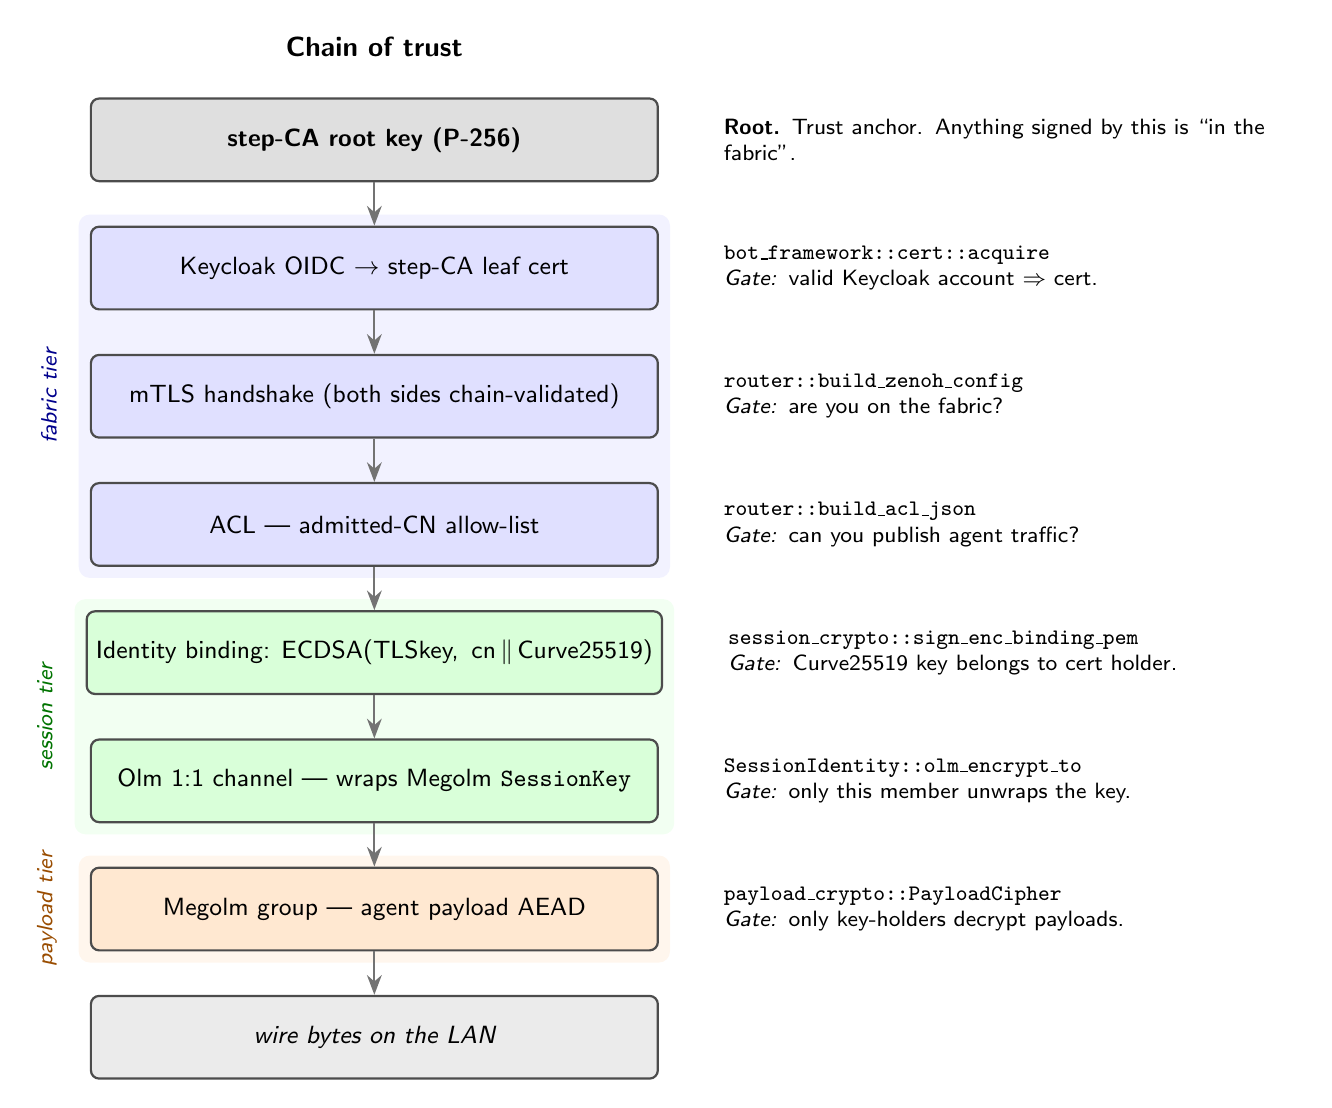
\begin{tikzpicture}[
    node distance=0.55cm,
    layer/.style={
      rectangle, draw=black!70, thick, rounded corners=3pt,
      minimum width=7.2cm, minimum height=1.05cm,
      font=\small\sffamily, align=center,
    },
    root/.style    ={layer, fill=gray!25,  font=\small\bfseries\sffamily},
    fabric/.style  ={layer, fill=blue!12},
    session/.style ={layer, fill=green!15},
    payload/.style ={layer, fill=orange!18},
    wire/.style    ={layer, fill=black!8,  font=\small\sffamily\itshape},
    annot/.style={font=\footnotesize\sffamily, align=left,
                  anchor=west, text width=7.2cm},
    arrow/.style={-{Stealth[length=2.5mm]}, thick, black!55},
]

\node[root]                       (L0) {step-CA root key (P-256)};
\node[fabric,  below=of L0]       (L1) {Keycloak OIDC $\to$ step-CA leaf cert};
\node[fabric,  below=of L1]       (L2) {mTLS handshake (both sides chain-validated)};
\node[fabric,  below=of L2]       (L3) {ACL --- admitted-CN allow-list};
\node[session, below=of L3]       (L4) {Identity binding: ECDSA(TLSkey,\, cn\,$\|$\,Curve25519)};
\node[session, below=of L4]       (L5) {Olm 1:1 channel --- wraps Megolm \texttt{SessionKey}};
\node[payload, below=of L5]       (L6) {Megolm group --- agent payload AEAD};
\node[wire,    below=of L6]       (W)  {wire bytes on the LAN};

\foreach \a/\b in {L0/L1, L1/L2, L2/L3, L3/L4, L4/L5, L5/L6, L6/W}
    \draw[arrow] (\a) -- (\b);

\node[annot, right=0.7cm of L0] {\textbf{Root.} Trust anchor.
                                  Anything signed by this is ``in the fabric''.};
\node[annot, right=0.7cm of L1] {\texttt{bot\_framework::cert::acquire} \\
                                  \emph{Gate:} valid Keycloak account $\Rightarrow$ cert.};
\node[annot, right=0.7cm of L2] {\texttt{router::build\_zenoh\_config} \\
                                  \emph{Gate:} are you on the fabric?};
\node[annot, right=0.7cm of L3] {\texttt{router::build\_acl\_json} \\
                                  \emph{Gate:} can you publish agent traffic?};
\node[annot, right=0.7cm of L4] {\texttt{session\_crypto::sign\_enc\_binding\_pem} \\
                                  \emph{Gate:} Curve25519 key belongs to cert holder.};
\node[annot, right=0.7cm of L5] {\texttt{SessionIdentity::olm\_encrypt\_to} \\
                                  \emph{Gate:} only this member unwraps the key.};
\node[annot, right=0.7cm of L6] {\texttt{payload\_crypto::PayloadCipher} \\
                                  \emph{Gate:} only key-holders decrypt payloads.};

\begin{scope}[on background layer]
  \node[fit=(L1)(L3), inner sep=4pt, fill=blue!5,   rounded corners=4pt] (fab)  {};
  \node[fit=(L4)(L5), inner sep=4pt, fill=green!5,  rounded corners=4pt] (sess) {};
  \node[fit=(L6),     inner sep=4pt, fill=orange!7, rounded corners=4pt] (pay)  {};
\end{scope}
\node[font=\footnotesize\sffamily\itshape, rotate=90, anchor=south, text=blue!55!black]
    at ($(fab.west)+(-0.15,0)$)  {fabric tier};
\node[font=\footnotesize\sffamily\itshape, rotate=90, anchor=south, text=green!45!black]
    at ($(sess.west)+(-0.15,0)$) {session tier};
\node[font=\footnotesize\sffamily\itshape, rotate=90, anchor=south, text=orange!60!black]
    at ($(pay.west)+(-0.15,0)$)  {payload tier};

\node[font=\sffamily\bfseries, above=0.4cm of L0] {Chain of trust};
\end{tikzpicture}


% ─── Figure 2: Session creation sequence ─────────────────────────────────────
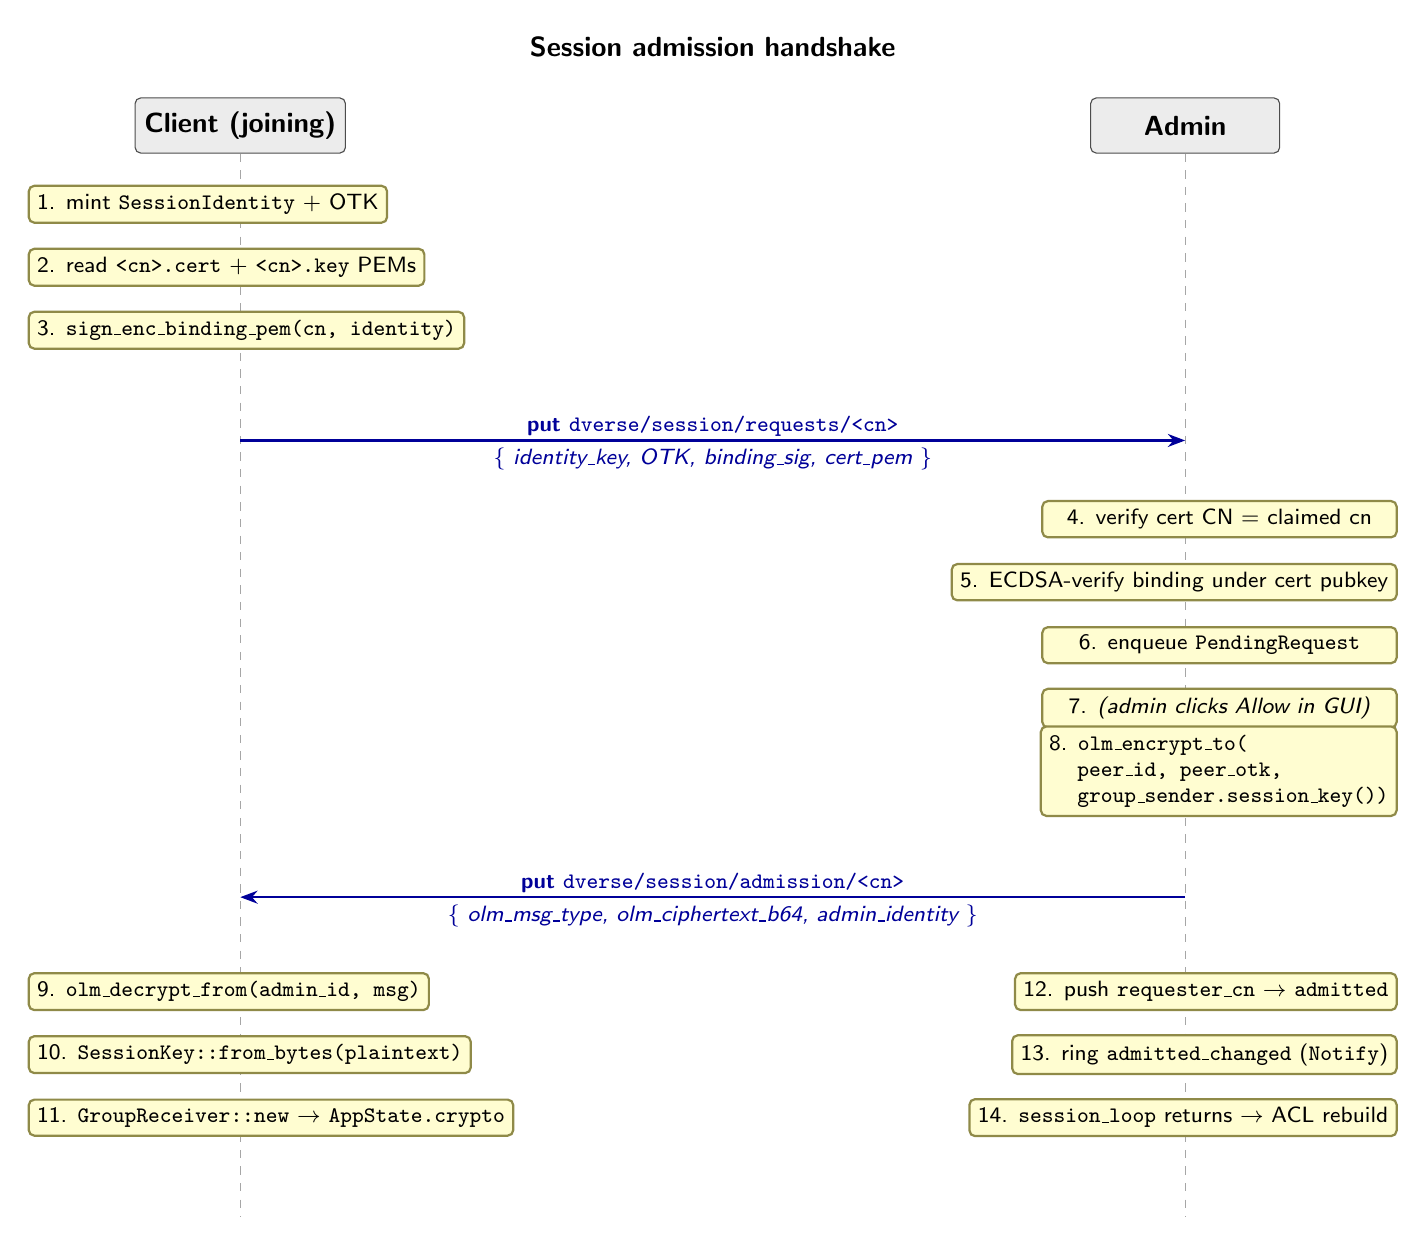
\begin{tikzpicture}[
    actor/.style={font=\sffamily\bfseries, align=center,
                  draw=black!70, fill=gray!15, rectangle, rounded corners=2pt,
                  minimum width=2.4cm, minimum height=0.7cm},
    action/.style={font=\footnotesize\sffamily, anchor=west,
                 fill=yellow!18, draw=yellow!50!black, thick,
                 rectangle, rounded corners=2pt, inner sep=3pt,
                 minimum width=4.5cm, align=left},
    actionR/.style={action, anchor=east},
    msg/.style={-{Stealth[length=2.2mm]}, thick, blue!60!black},
    msglabel/.style={font=\footnotesize\sffamily\bfseries, midway, above, fill=white, inner sep=1pt},
    msgpayload/.style={font=\footnotesize\sffamily\itshape, midway, below=0.5mm, fill=white, inner sep=1pt},
    life/.style={dashed, gray!70},
]
\node[actor] (C)  at (0, 0)  {Client (joining)};
\node[actor] (A)  at (12, 0) {Admin};

\draw[life] (C.south) -- ++(0,-13.5);
\draw[life] (A.south) -- ++(0,-13.5);

\node[action] at (-2.7, -1.0) {1. mint \texttt{SessionIdentity} + OTK};
\node[action] at (-2.7, -1.8) {2. read \texttt{<cn>.cert} + \texttt{<cn>.key} PEMs};
\node[action] at (-2.7, -2.6) {3. \texttt{sign\_enc\_binding\_pem(cn, identity)}};

\draw[msg] (C |- 0,-4.0) -- (A |- 0,-4.0)
    node[msglabel] {put \texttt{dverse/session/requests/<cn>}}
    node[msgpayload] {\{ identity\_key, OTK, binding\_sig, cert\_pem \}};

\node[actionR] at (14.7, -5.0) {4. verify cert CN $=$ claimed cn};
\node[actionR] at (14.7, -5.8) {5. ECDSA-verify binding under cert pubkey};
\node[actionR] at (14.7, -6.6) {6. enqueue \texttt{PendingRequest}};
\node[actionR] at (14.7, -7.4) {7. \emph{(admin clicks Allow in GUI)}};
\node[actionR] at (14.7, -8.2) {8. \texttt{olm\_encrypt\_to(}\\
                                \hspace*{1.2em}\texttt{peer\_id, peer\_otk,}\\
                                \hspace*{1.2em}\texttt{group\_sender.session\_key()}\texttt{)}};

\draw[msg] (A |- 0,-9.8) -- (C |- 0,-9.8)
    node[msglabel] {put \texttt{dverse/session/admission/<cn>}}
    node[msgpayload] {\{ olm\_msg\_type, olm\_ciphertext\_b64, admin\_identity \}};

\node[action] at (-2.7, -11.0) {9. \texttt{olm\_decrypt\_from(admin\_id, msg)}};
\node[action] at (-2.7, -11.8) {10. \texttt{SessionKey::from\_bytes(plaintext)}};
\node[action] at (-2.7, -12.6) {11. \texttt{GroupReceiver::new} $\to$ \texttt{AppState.crypto}};

\node[actionR] at (14.7, -11.0) {12. push \texttt{requester\_cn} $\to$ \texttt{admitted}};
\node[actionR] at (14.7, -11.8) {13. ring \texttt{admitted\_changed} (\texttt{Notify})};
\node[actionR] at (14.7, -12.6) {14. \texttt{session\_loop} returns $\to$ ACL rebuild};

\node[font=\sffamily\bfseries, above=0.4cm of C, xshift=6cm] {Session admission handshake};
\end{tikzpicture}

\end{document}
